%-------------
% PACKAGES %%
%-------------
\documentclass[12pt]{article}
\usepackage[english]{babel}
\usepackage[utf8x]{inputenc}
\usepackage{amsmath}
\usepackage{float}
\usepackage{hyperref}
\usepackage{graphicx}
\usepackage{listings}
\usepackage[colorinlistoftodos]{todonotes}
\usepackage[nottoc,numbib]{tocbibind}
\usepackage[parfill]{parskip}
\usepackage{changepage}
\usepackage{subcaption}
\usepackage{changepage}
\usepackage{listings}
\usepackage{color}
\usepackage{float}
\usepackage[htt]{hyphenat}
%\usepackage{minted}

\definecolor{dkgreen}{rgb}{0,0.6,0}
\definecolor{gray}{rgb}{0.5,0.5,0.5}
\definecolor{mauve}{rgb}{0.58,0,0.82}

\lstset{%frame=tb,
  language=C,
  aboveskip=3mm,
  belowskip=3mm,
  showstringspaces=false,
  columns=flexible,
  basicstyle={\small\ttfamily},
  numbers=none,
  numberstyle=\tiny\color{gray},
  keywordstyle=\color{blue},
  commentstyle=\color{dkgreen},
  stringstyle=\color{mauve},
  breaklines=false,
  breakatwhitespace=false,
  tabsize=4,
  morekeywords={FIR_H_BUFFER,dsp16_t,dsp16_filt_iirpart}
}

\lstset{emph={%  
    DSP16_Q,H_SIZE%
    },emphstyle={\color{mauve}}%
}

\title{Hochschule Bonn-Rhein-Sieg}

\begin{document}

%-------------------------
%	uncomment irrelevant 
%	parts, like logo etc
%-------------------------
\pagenumbering{Alph}
\begin{titlepage}

\newcommand{\HRule}{\rule{\linewidth}{0.5mm}} % Defines a new command for the horizontal lines, change thickness here

\begin{center}
%---------------------
%	HEADING SECTIONS
%---------------------
\textsc{\LARGE Hochschule Bonn-Rhein-Sieg}\\[1.5cm] % Name of your university/college
\textsc{\Large Multi-Agent and Agent Systems}\\[0.5cm] % Major heading such as course name
\textsc{\large Team : Right brothers}\\[0.5cm] % Minor heading such as course title

%------------------
%	TITLE SECTION
%------------------
\HRule \\[0.4cm]
{ \huge \bfseries Flying Saucers Bakery}\\[0.4cm] % Title of your document
\HRule \\[1.5cm]
 
%--------------------
%	AUTHOR SECTION
%--------------------
 %\begin{minipage}{1.4\textwidth}
 %\begin{flushleft} 

\large\emph{Authors:}\\ Arun Rajendra Prabhu\\ Dharmin Bakaraniya\\ Md Zahiduzzaman\\[1.0cm]%
%\large\emph{Collaborated with:}\\Collaborator\\[1cm]
                        		% \\ [1.0cm]%

 %\end{flushleft}
 %\end{minipage}

%---------------------
%	Supervisor
%---------------------
 %\begin{minipage}{0.4\textwidth}
 %\begin{flushright} \large
 %\emph{Supervisor:} \\
 %Dr. James \textsc{Smith} % Supervisor's Name
 %\end{flushright}
 %\end{minipage}\\[2cm]

% If you don't want a supervisor, uncomment the two lines below and remove the section above
%\Large \emph{Author:}\\
%John \textsc{Smith}\\[3cm] % Your name

{\large \today}\\[1cm] % Date

%----------
%	LOGO 
%----------

\includegraphics[width=3.7in]{Logo.png}\\%[1cm]
\end{center}
\end{titlepage}
\pagenumbering{arabic}
\pagebreak
%-------------------------
%	Table of Contents
%-------------------------
\tableofcontents
\pagebreak
%-------------------------
%       Main Text
%-------------------------
\section*{Introduction:}

The overall architecture diagram describing the deligation of tasks in the bakery is provided by the figure~\ref{fig:1}.

\begin{figure}[H]
  \centering
  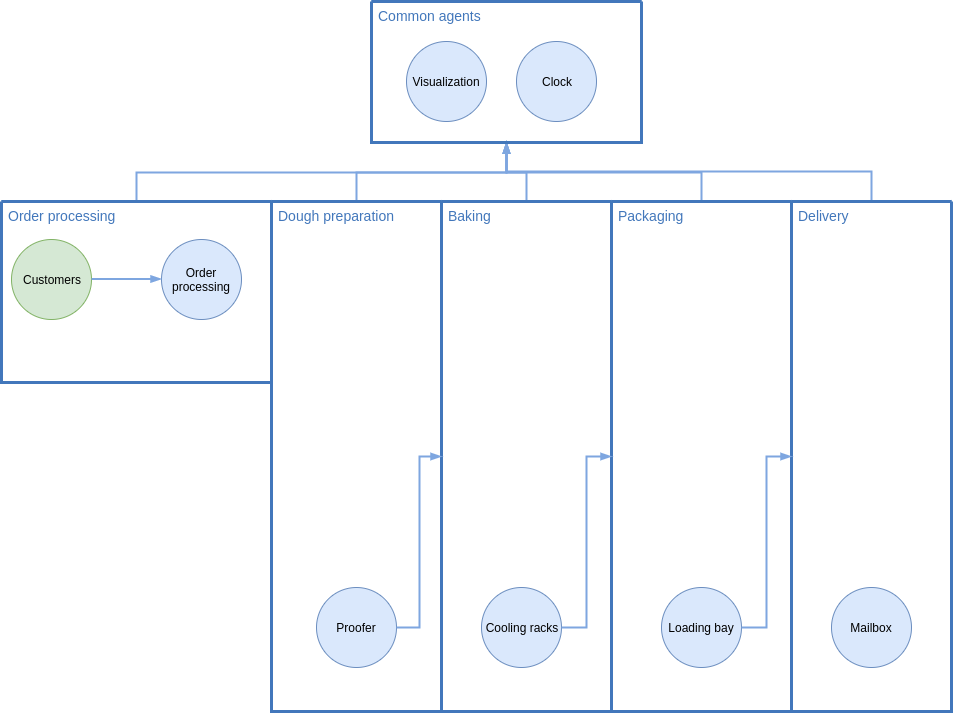
\includegraphics[width=0.8\textwidth]{Architecture.png}
  \caption{Architecture Diagram}
  \label{fig:1}
\end{figure}

The right brothers team was responsible to provide the \textbf{baking} and \textbf{packaging} stages. In addition to these stages, it was also responsible for providing the \textbf{base agent}, \textbf{time keeper} agent and \textbf{board visualization} feature. These agents fall in the common agents catagory and we will look at each one of them in detail in the coming sections.

With figure~\ref{fig:1} as the starting point, we created a component diagram, figure~\ref{fig:2} to describe the relationship between the agents in different stages. This diagram was created from the perspective of the stages which are under the right brother's responsibility, hence the only the interface agents of the other stages are represented in the diagram.
 
\begin{figure}[H]
  \centering
  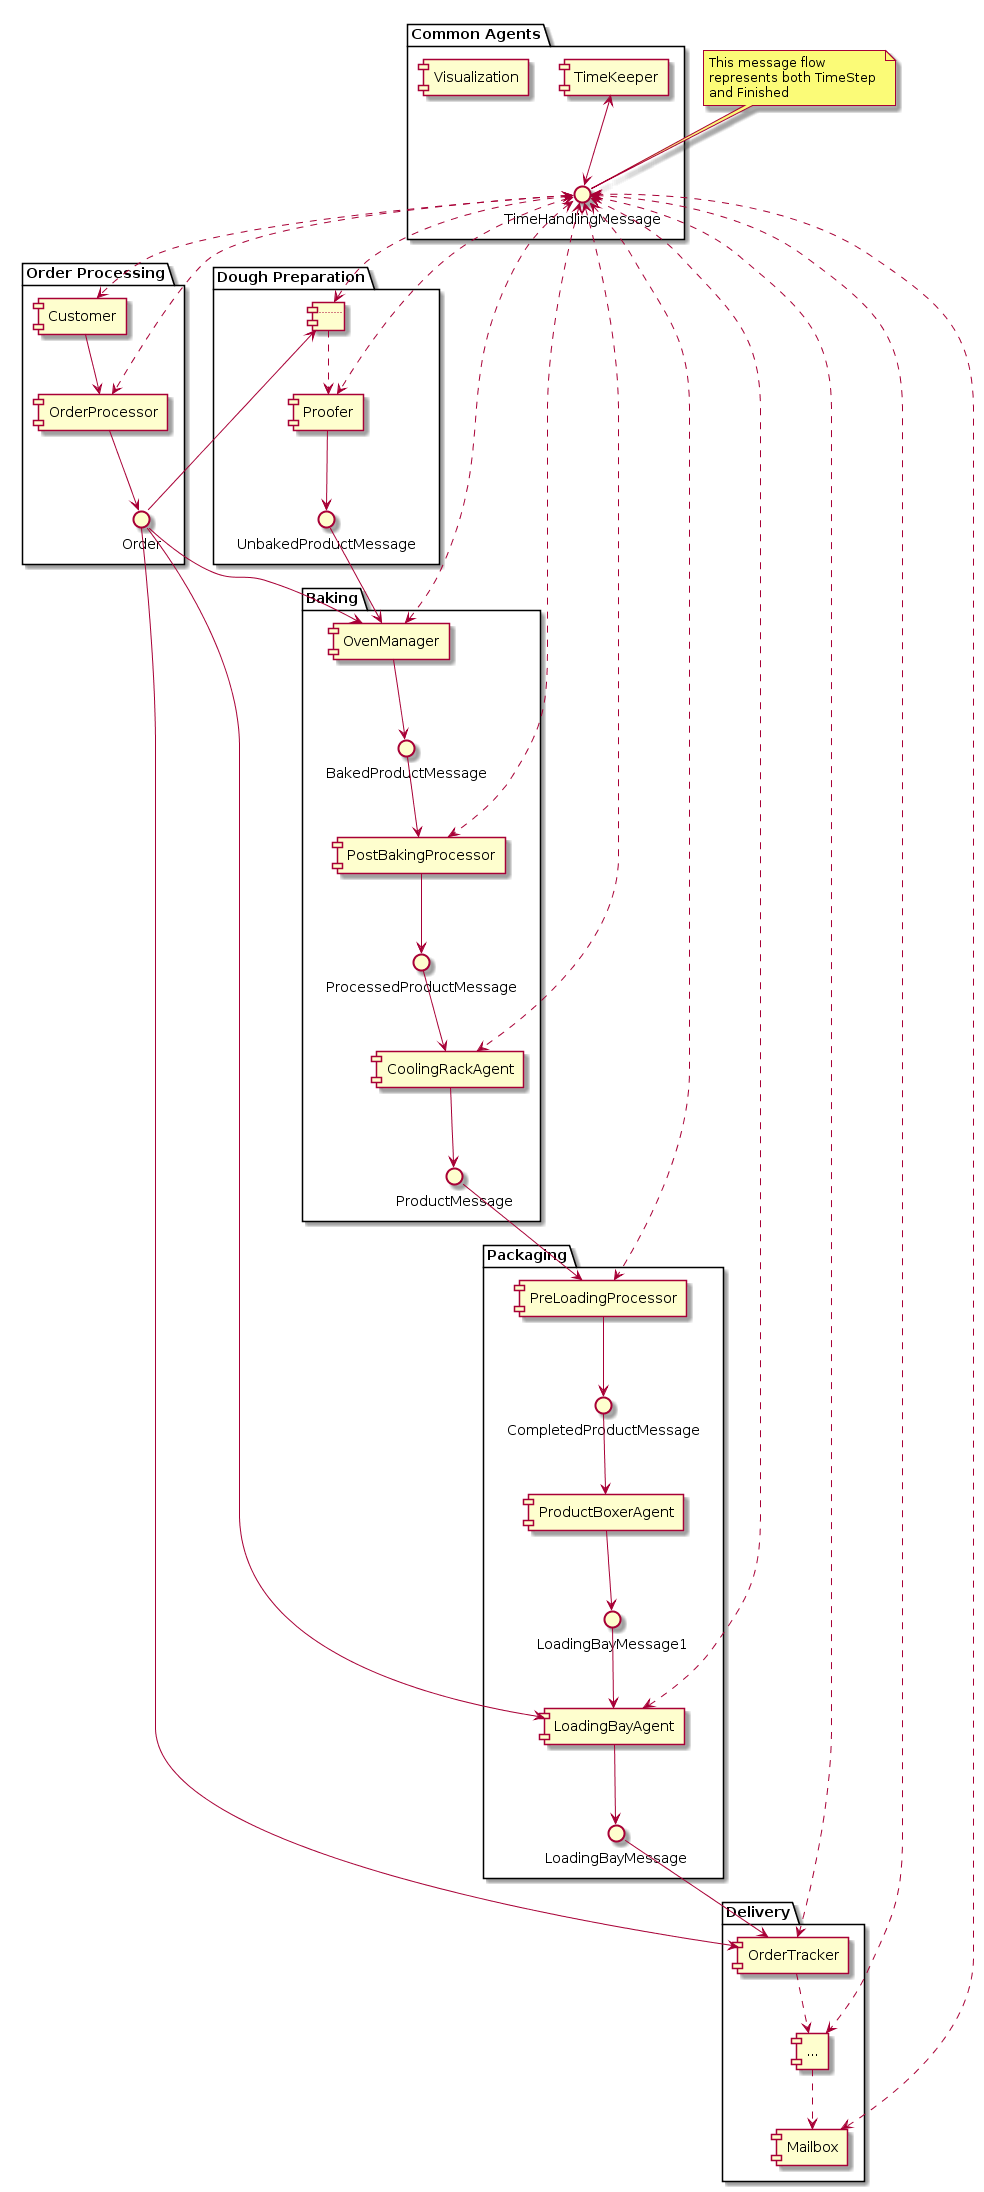
\includegraphics[width=0.7\textwidth]{component_diagram.png}
  \caption{Component diagram representation}
  \label{fig:2}
\end{figure}

All the agents in our stages are created statically at startup. 
To illustrate this decision, consider the baking stage. Each bakery has a fixed number of ovens. In our design, we have a single agent called as OvenManager looking after all the ovens. Hence as per our design, it does not make sense to use dynamic agent creation for OvenManager. Also static agent creation, simplifies the overall interoperability to a cetain extent.

\section{Baking Stage:}
\begin{itemize}
    \item \textbf{OvenManager}: 
 We assign a single Agent to manage all the ovens in the bakery.
 It receives the \texttt{Order} from \texttt{OrderProcessor} agent. 
 It receives \texttt{UnbakedProductMessage} from \texttt{Proofer}.
 It bakes the products it received from \texttt{Proofer} and sends \texttt{BakedProductMessage} to \texttt{PostBakingProcessor}.
 It aggregates products of same type if the product is not being baked. 
    \item \textbf{PostBakingProcessor}:
 It receives \texttt{BakedProductMessage} from \texttt{OvenManager}.
 It processes all the steps in the recipe of that product which occur between \texttt{Baking} and \texttt{Cooling} steps. 
 It sends the \texttt{ProcessedProductMessage} to \texttt{CoolingRackAgent}.
    \item \textbf{CoolingRackAgent}:
 It receives \texttt{ProcessedProductMessage} from \texttt{PostBakingProcessor}.
 It performs cooling step of the recipe corresponding to that product.
 It sends \texttt{ProductMessage} to \texttt{PreLoadingProcessor} in the packaging stage.
\end{itemize}
\section{Packaging Stage:}
\begin{itemize}
    \item \textbf{PreLoadingProcessor}:
 It recieves \texttt{ProductMessage} from \texttt{CoolingRackAgent} from Baking stage.
 It performs all steps in recipe of that product which lie between \texttt{Cooling} and \texttt{Packaging}.
 It sends \texttt{CompletedProductMessage} to \texttt{ProductBoxerAgent}.
	\item \textbf{ProductBoxerAgent}: It receives \texttt{CompletedProductMessage} from the \texttt{PreLoadingProcessor}. It also receives the \texttt{Order} from \texttt{OrderProcessor}. It then prioritizes the orders based on the delivery times. It supports two types of priorities,
\begin{itemize}
\item Hard priority: Waits for the entire order of higher priority is completed before it moves on to process the next high priority order.
\item Soft priority: Checks if the products available in the inventory can be used to satisfy the pending orders according to their priority. If suppose there are 5 donuts in inventory and order1(high priority) needs 10 donuts and order2(lower priority) needs 5 donuts, then the 5 donuts are used to satisfy order2. However if there were 10 donuts in the inventory then the 10 donuts would have been used to satisfy order1.\
\end{itemize}
\texttt{LoadingBayMessage} is sent to the \texttt{LoadingBay} agent under two conditions,
\begin{itemize}
\item If a box is filled.
\item If a box is not full, however, all the required number of items of a product type in an order have been received.
\end{itemize}
    \item \textbf{LoadingBayAgent}:
 It recieves \texttt{LoadingBayMessage} from \\ \texttt{ProductBoxerAgent}.
 It then checks for order completion. If any orders are complete, it sends the  message to the \texttt{OrderTracking/OrderAggregator} agent of the \texttt{Delivery Stage}.   
\end{itemize}

\section{Common Agents:}
\begin{itemize}
    \item \textbf{TimeKeeper}: 
 It is responsible for the movement of time in the entire bakery eco-system.
 This is responsible for providing all the other agents with a common time reference so that everyone are in sync except the visualization agents.
 This also gets feedback from all the agents about the status of their tasks.
 If all the agents are done with whatever task they were supposed to finish in the time step, the TimeKeeper increments the time step. 
 It is also responsible for shutting down the platform when the simulation time ends.
\item \textbf{BaseAgent}:
BaseAgent is a parent to all agents in bakery simulation.
It is mainly responsible for registering the agent to yellow pages and talking to TimeKeeper.
It is also responsible for sending the message to visualization agents.
Every agent that inherits BaseAgent has to call \texttt{finished} when their task is finished for that time step.
\item \textbf{Visualization}:
VisualizationAgent receives the output messages of the interface agents. It is a JADE agent extended from \textbf{BaseAgent}. It creates an instance of JavaFX application instance \textbf{Visualizer} during initialization and forwards all interface agent messages to the Visualizer instance.
Please refer Figure~\ref{fig:visualizer-ui} for a snapshot of the visualiser gui in action and refer 
Figure~\ref{fig:class_diagram_for_visualiser} for the class diagram of the visualiser agent.
\begin{figure}[H]
	\centering
	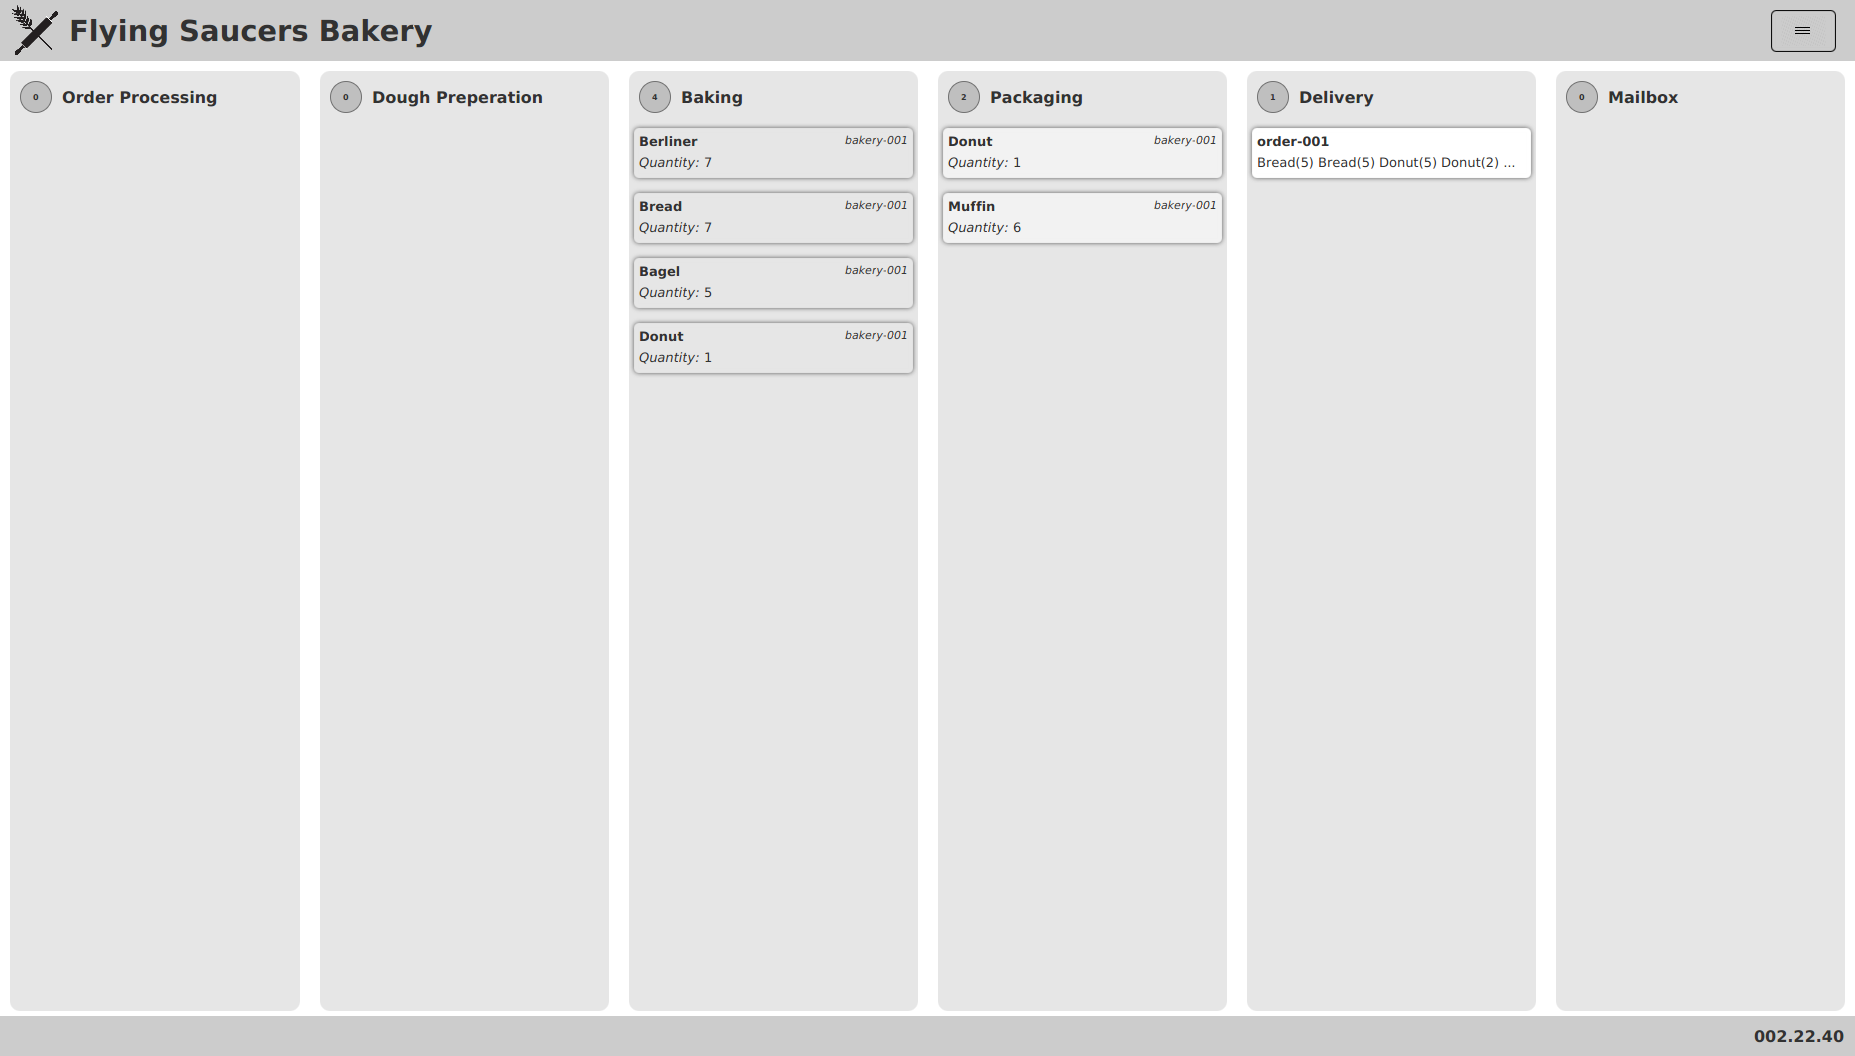
\includegraphics[width=1.0\linewidth]{visualizer-ui.png}
    \caption{Board visualization in progress}\label{fig:visualizer-ui}
\end{figure}
\begin{figure}[H]
    \centering
    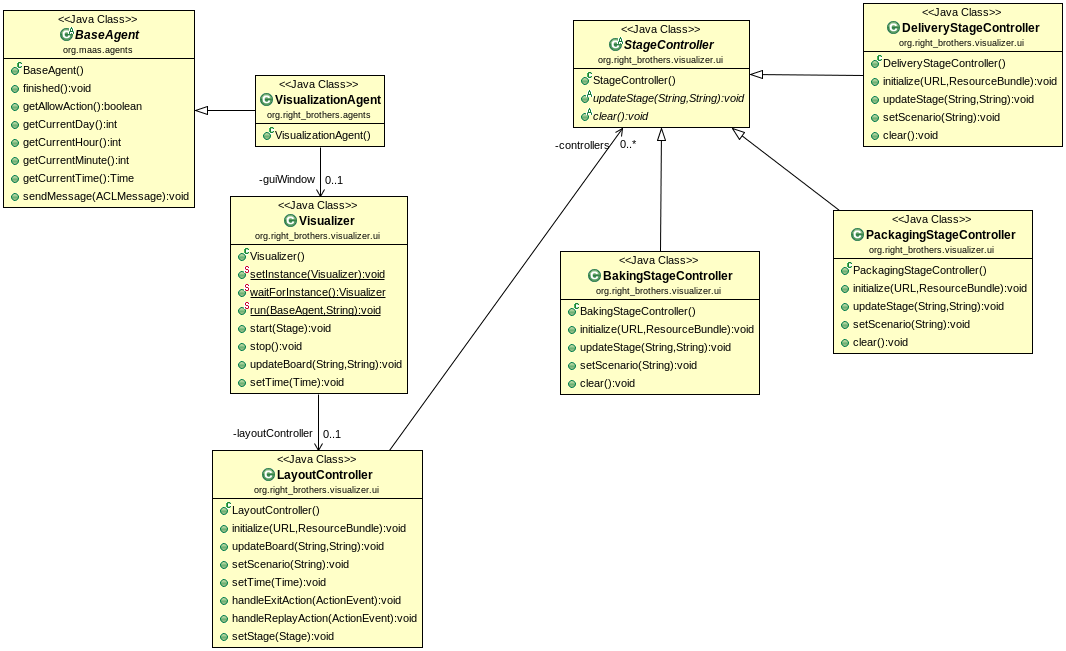
\includegraphics[width=1.0\linewidth]{class-diagram.png}
    \caption{Class diagram of the major classes of the visualizer}\label{fig:class_diagram_for_visualiser}
\end{figure}

\end{itemize}

\section{Mockup Agents:}
For testing the individual stages for proper functioning, we create a number of agents basically as mockup agents to provided the necessary input messages to the interface messages of our stages. These are listed below along with their functionality.
\begin{itemize}
    \item \textbf{DummyAgent}:
        The purpose of this agent was to test the TimeKeeper agent. It prints a message every time step
        till the platform shuts down.
    \item \textbf{DummyCoolingRackAgent}:
        This dummy agent get the order messages from order processing agent and creates ProductMessage
        objects. This product message is converted into a json string message and sent to PreLoadingBayAgent.
        This dummy is used in the test for packaging stage.
    \item \textbf{DummyOrderProcessor}:
        This dummy agent reads a client.json file from a scenario directory and create order messages
        from that information. This order message is then sent to all the agents of its bakery. The 
        dummy order processor takes all the order for its bakery so there cannot be multiple order processing 
        agent reading the same file.
    \item \textbf{DummyProofer}:
        Similar to DummyCoolingRackAgent, this agent receives order messages from order processing 
        agent and converts the order to UnbakedProductMessage and sends it to the OvenManager of its 
        bakery.
    \item \textbf{DummyReceiverAgent}:
        This agent is made for the sole purpose of receiving INFORM messages from a particular agent.
        It takes 3 arguments, namely, guid of the bakery it is part of, the name of the agent it will
        receive messages from and the conversation id of those messages. This agent is also used for 
        testing different stages. It is the last agent in the chain and once it receives a message, 
        we assert that the stage is working correctly.
\end{itemize}

Following section will provided class descriptions for the different agents discussed in this section.

\newpage{}
\section{Class descriptions}%
\label{sec:agent_descriptions}

\subsection{TimeKeeper}
\begin{itemize}
    \item \textbf{Stage}: Common Agent
    \item \textbf{Agent/Object}: Agent
    \item \textbf{Static/Dynamic}: Static
    \item \textbf{Behaviour}: SendTimeStep (OneShot), TimeStepConfirmationBehaviour (Cyclic)
    \item \textbf{Messages in}: 
        \begin{itemize}
            \item  finished (Sender: all agents)
        \end{itemize}
    \item \textbf{Messages out}:
        \begin{itemize}
            \item  TimeStep (Receiver: all agents)
        \end{itemize}
\end{itemize}
%\newpage{}

\subsection{BaseAgent}
\begin{itemize}
    \item \textbf{Stage}: NA
    \item \textbf{Agent/Object}: Agent
    \item \textbf{Static/Dynamic}: Static  
    \item \textbf{Behaviour}: PermitAction (Cyclic)
    \item \textbf{Messages in}:
        \begin{itemize}
            \item  TimeStep (Sender: TimeKeeper)
        \end{itemize}
    \item \textbf{Messages out}:
        \begin{itemize}
            \item  finished (Receiver: TimeKeeper)
            \item  all messages(Receiver: Visualization Agents)
        \end{itemize}
\end{itemize}
\newpage{}

\subsection{Visualization agent}
\begin{itemize}
    \item \textbf{Stage}: Common Agents 
    \item \textbf{Agent/Object}: Agent
    \item \textbf{Static/Dynamic}: Static
    \item \textbf{Behaviour}: MessageServer (Cyclic)
    \item \textbf{Messages in}:
        \begin{itemize}
            \item  all messages (Sender: all agents)
        \end{itemize}
\end{itemize}
%\newpage{}

\subsection{OvenManager}
\begin{itemize}
    \item \textbf{Stage}: Baking 
    \item \textbf{Agent/Object}: Agent 
    \item \textbf{Static/Dynamic}: Static
    \item \textbf{Behaviour}: Bake (Cyclic), OrderServer (Cyclic), UnbakedProductsServer (Cyclic) 
    \item \textbf{Messages in}:
        \begin{itemize}
            \item  Order (Sender: OrderProcessor)
            \item  UnbakedProductMessage (Sender: Proofer)
        \end{itemize}
    \item \textbf{Messages out}:
        \begin{itemize}
            \item  BakedProductMessage (Receiver: PostBakingProcessor)
        \end{itemize}
\end{itemize}
\newpage{}

\subsection{PostBakingProcessor}
\begin{itemize}
    \item \textbf{Stage}: Baking
    \item \textbf{Agent/Object}: Agent 
    \item \textbf{Static/Dynamic}: Static
    \item \textbf{Behaviour}: BakedProductsServer (Cyclic), Process (Cyclic)
    \item \textbf{Messages in}:
        \begin{itemize}
            \item  BakedProductMessage (Sender: OvenManager)
        \end{itemize}
    \item \textbf{Messages out}:
        \begin{itemize}
            \item  ProcessedProductMessage (Receiver: CoolingRackAgent)
        \end{itemize}
\end{itemize}
%\newpage{}

\subsection{CoolingRackAgent}
\begin{itemize}
    \item \textbf{Stage}: Baking
    \item \textbf{Agent/Object}: Agent
    \item \textbf{Static/Dynamic}: Static
    \item \textbf{Behaviour}: ProcessedProductServer (Cyclic), CoolProducts (Cyclic)
    \item \textbf{Messages in}:
        \begin{itemize}
            \item ProcessedProductMessage (Sender: PostBakingProcessor)
        \end{itemize}
    \item \textbf{Messages out}:
        \begin{itemize}
            \item ProductMessage (Receiver: PreLoadingProcessor)
        \end{itemize}
\end{itemize}
\newpage{}

\subsection{PreLoadingProcessor}
\begin{itemize}
    \item \textbf{Stage}: Packaging
    \item \textbf{Agent/Object}: Agent
    \item \textbf{Static/Dynamic}: Static
    \item \textbf{Behaviour}: Process (Cyclic), CooledProductServer (Cyclic), OrderServer (Cyclic)
    \item \textbf{Messages in}:
        \begin{itemize}
            \item ProductMessage (Sender: CoolingRackAgent)
            \item Order (Sender: OrderProcessor)
        \end{itemize}
    \item \textbf{Messages out}:
        \begin{itemize}
            \item CompletedProductMessage (Receiver: LoadingBayAgent)
        \end{itemize}
\end{itemize}

\subsection{ProductBoxerAgent}
\begin{itemize}
    \item \textbf{Stage}: Packaging
    \item \textbf{Agent/Object}: Agent
    \item \textbf{Static/Dynamic}: Static
    \item \textbf{Behaviour}: OrderReceiver (Cyclic), CompletedProductReceiver (Cyclic)
    \item \textbf{Messages in}:
        \begin{itemize}
            \item CompletedProductMessage (Sender: PreLoadingProcessor)
        \end{itemize}
    \item \textbf{Messages out}:
        \begin{itemize}
            \item LoadingBayMessage (Receiver: LoadingBayAgent)
        \end{itemize}
\end{itemize}

\newpage{}

\subsection{LoadingBayAgent}
\begin{itemize}
    \item \textbf{Stage}: Packaging
    \item \textbf{Agent/Object}: Agent
    \item \textbf{Static/Dynamic}: Static
    \item \textbf{Behaviour}: OrderDetailsReceiver (Cyclic), ProductDetailsReceiver (Cyclic)
    \item \textbf{Messages in}:
        \begin{itemize}
            \item LoadingBayAgent (Sender: ProductBoxerAgent)
        \end{itemize}
    \item \textbf{Messages out}:
        \begin{itemize}
            \item LoadingBayMessage (Receiver: OrderTracker/OrderAggregator)
        \end{itemize}
\end{itemize}

\section{Message Object Description}
\subsection{UnbakedProductMessage}
\begin{itemize}
\item Recipient: OvenManager(Baking Stage)
\item Sender: Proofer(Dough Preparation Stage)
\item Class description:
\begin{lstlisting}[language=Java]
public class UnbakedProductMessage implements java.io.Serializable {
    private String productType;
    private Vector<String> guids; 
    private Vector<Integer> productQuantities;
    
	public UnbakedProductMessage() {
        this.guids = new Vector<String> ();
        this.productQuantities = new Vector<Integer> ();
	}

    public void setProductType(String productType) {
        this.productType = productType;
    }

    public String getProductType() {
        return productType;
    }

    public void setGuids(Vector<String> guids) {
        this.guids = guids;
    }

    public Vector<String> getGuids() {
        return guids;
    }

    public void setProductQuantities(Vector<Integer> productQuantities) {
        this.productQuantities = productQuantities;
    }

    public Vector<Integer> getProductQuantities() {
        return productQuantities;
    }
}
\end{lstlisting} 

\end{itemize}
\subsection{BakedProductMessage}
\begin{itemize}
\item Recipient: PostBakingProcessor(Baking Stage)
\item Sender: OvenManager(Baking Stage)
\item Class description:
\begin{lstlisting}[language=Java]
public class BakedProductMessage implements java.io.Serializable {
    private String guid;
    private int coolingDuration;
    private Vector<Step> intermediateSteps;
    private int quantity;
    
	public BakedProductMessage() {
        this.intermediateSteps = new Vector<Step> ();
	}
    public void setGuid(String id) {
        this.guid = id;
    }

    public String getGuid() {
        return this.guid;
    }

    public void setCoolingDuration(int coolingDuration) {
        this.coolingDuration = coolingDuration;
    }

    public int getCoolingDuration() {
        return coolingDuration;
    }

    public void setQuantity(int quantity) {
        this.quantity = quantity;
    }

    public int getQuantity() {
        return quantity;
    }

    public void setIntermediateSteps(Vector<Step> intermediateSteps) {
        this.intermediateSteps = intermediateSteps;
    }

    public Vector<Step> getIntermediateSteps() {
        return intermediateSteps;
    }
}
\end{lstlisting}
\end{itemize}
\subsection{ProcessedProductMessage}
\begin{itemize}
\item Recipient: CoolingRackAgent(Baking Stage)
\item Sender: PostBakingProcessor(Baking Stage)
\item Class description:
\begin{lstlisting}[language=Java]
public class ProcessedProductMessage implements java.io.Serializable {
    private String guid;
    private int coolingDuration;
    private int quantity;
    
    public void setGuid(String id) {
        this.guid = id;
    }

    public String getGuid() {
        return this.guid;
    }

    public void setCoolingDuration(int coolingDuration) {
        this.coolingDuration = coolingDuration;
    }

    public int getCoolingDuration() {
        return coolingDuration;
    }

    public void setQuantity(int quantity) {
        this.quantity = quantity;
    }

    public int getQuantity() {
        return quantity;
    }

}
\end{lstlisting}
\end{itemize}
\subsection{ProductMessage}
\begin{itemize}
\item Recipient: PreLoadingProcessor(Packaging Stage)
\item Sender: CoolingRackAgent(Baking Stage)
\item Class description:
\begin{lstlisting}[language=Java]
public class ProductMessage implements java.io.Serializable {
    private Hashtable<String,Integer> products;
    
    public ProductMessage() {
        this.setProducts(new Hashtable<>());
    }

    public void setProducts(Hashtable<String,Integer> products) {
        this.products = products;
    }

    public Hashtable<String,Integer> getProducts() {
        return products;
    }
}
\end{lstlisting}
\end{itemize}
\subsection{CompletedProductMessage}
\begin{itemize}
\item Recipient: ProductBoxerAgent(Packaging Stage)
\item Sender: PreLoadingProcessor(Packaging Stage)
\item Class description:
\begin{lstlisting}[language=Java]
public class CompletedProductMessage implements java.io.Serializable {
    private String guid;
    private int quantity;
    
    public void setGuid(String id) {
        this.guid = id;
    }

    public String getGuid() {
        return this.guid;
    }

    public void setQuantity(int quantity) {
        this.quantity = quantity;
    }

    public int getQuantity() {
        return quantity;
    }

}
\end{lstlisting}
\end{itemize}
\subsection{LoadingBayMessage}
\begin{itemize}
\item Recipient: LoadingBayAgent(Packaging Stage)
\item Sender: ProductBoxerAgent(Packaging Stage)
\item Class description:
\begin{lstlisting}[language=Java]
public class LoadingBayMessage {
	private String orderId;
	private List<LoadingBayBox> boxes;
	
	public LoadingBayMessage() {
		boxes = new ArrayList<LoadingBayBox>();
	}
	
	public LoadingBayMessage(String orderId, List<LoadingBayBox> boxes) {
		this();
		
		this.orderId = orderId;
		this.boxes = boxes;
	}
	@JsonProperty("OrderID")
	public String getOrderId() {
		return orderId;
	}

	public void setOrderId(String orderId) {
		this.orderId = orderId;
	}
	@JsonProperty("Boxes")
	public List<LoadingBayBox> getBoxes() {
		return boxes;
	}
	public void setBoxes(List<LoadingBayBox> boxes) {
		this.boxes = boxes;
	}
}

\end{lstlisting}
\end{itemize}

\section{Testing}%
\label{sec:testing}
\begin{itemize}
    \item For testing TimeKeeper \\\texttt{gradle run}
    \item For testing baking stage \\\texttt{gradle run --args="-baking"}
    \item For testing packaging stage \\\texttt{gradle run --args="-packaging"}
    \item For testing baking and packaging stage \\\texttt{gradle run --args="-baking -packaging"}
    \item For testing baking and packaging and visualisation stage \\\texttt{gradle run --args="-baking -packaging -visualization"}
\end{itemize}






\bibliography{refs}
\bibliographystyle{IEEEtran}

\end{document}
